\PassOptionsToPackage{unicode=true}{hyperref} % options for packages loaded elsewhere
\PassOptionsToPackage{hyphens}{url}
%
\documentclass[]{article}
\usepackage{lmodern}
\usepackage{amssymb,amsmath}
\usepackage{ifxetex,ifluatex}
\usepackage{fixltx2e} % provides \textsubscript
\ifnum 0\ifxetex 1\fi\ifluatex 1\fi=0 % if pdftex
  \usepackage[T1]{fontenc}
  \usepackage[utf8]{inputenc}
  \usepackage{textcomp} % provides euro and other symbols
\else % if luatex or xelatex
  \usepackage{unicode-math}
  \defaultfontfeatures{Ligatures=TeX,Scale=MatchLowercase}
\fi
% use upquote if available, for straight quotes in verbatim environments
\IfFileExists{upquote.sty}{\usepackage{upquote}}{}
% use microtype if available
\IfFileExists{microtype.sty}{%
\usepackage[]{microtype}
\UseMicrotypeSet[protrusion]{basicmath} % disable protrusion for tt fonts
}{}
\IfFileExists{parskip.sty}{%
\usepackage{parskip}
}{% else
\setlength{\parindent}{0pt}
\setlength{\parskip}{6pt plus 2pt minus 1pt}
}
\usepackage{hyperref}
\hypersetup{
            pdftitle={The Measure of the Archive: The Robustness of Network Analysis in the Light of Missing Data},
            pdfborder={0 0 0},
            breaklinks=true}
\urlstyle{same}  % don't use monospace font for urls
\usepackage[margin=1in]{geometry}
\usepackage{longtable,booktabs}
% Fix footnotes in tables (requires footnote package)
\IfFileExists{footnote.sty}{\usepackage{footnote}\makesavenoteenv{longtable}}{}
\usepackage{graphicx,grffile}
\makeatletter
\def\maxwidth{\ifdim\Gin@nat@width>\linewidth\linewidth\else\Gin@nat@width\fi}
\def\maxheight{\ifdim\Gin@nat@height>\textheight\textheight\else\Gin@nat@height\fi}
\makeatother
% Scale images if necessary, so that they will not overflow the page
% margins by default, and it is still possible to overwrite the defaults
% using explicit options in \includegraphics[width, height, ...]{}
\setkeys{Gin}{width=\maxwidth,height=\maxheight,keepaspectratio}
\setlength{\emergencystretch}{3em}  % prevent overfull lines
\providecommand{\tightlist}{%
  \setlength{\itemsep}{0pt}\setlength{\parskip}{0pt}}
\setcounter{secnumdepth}{5}
% Redefines (sub)paragraphs to behave more like sections
\ifx\paragraph\undefined\else
\let\oldparagraph\paragraph
\renewcommand{\paragraph}[1]{\oldparagraph{#1}\mbox{}}
\fi
\ifx\subparagraph\undefined\else
\let\oldsubparagraph\subparagraph
\renewcommand{\subparagraph}[1]{\oldsubparagraph{#1}\mbox{}}
\fi

% set default figure placement to htbp
\makeatletter
\def\fps@figure{htbp}
\makeatother

\usepackage{xcolor}
\usepackage{setspace}\doublespacing
\usepackage{booktabs}
\usepackage{longtable}
\usepackage{array}
\usepackage{multirow}
\usepackage{wrapfig}
\usepackage{float}
\usepackage{colortbl}
\usepackage{pdflscape}
\usepackage{tabu}
\usepackage{threeparttable}
\usepackage{threeparttablex}
\usepackage[normalem]{ulem}
\usepackage{makecell}
\usepackage{xcolor}

\title{The Measure of the Archive: The Robustness of Network Analysis in the Light of Missing Data}
\author{}
\date{\vspace{-2.5em}}

\begin{document}
\maketitle

\hypertarget{introduction}{%
\section{Introduction}\label{introduction}}

The archives that historians work with are filled with traces of damaged, lost, and destroyed letters, which, had they survived, might have profoundly changed established historical narratives. Sometimes these archival gaps are created during the lifetime of the individual in question: fleeing persecution in Catholic-run Bohemia, the theologian, pedagogue and minister Jan Comenius took refuge in Leszno in Poland, where he administered a school and was made the leader of the Moravian and Bohemian churches. In 1656, during the Swedish invasion of Poland, Comenius had declared his support for the Swedish side. In retaliation, the Polish Catholic partisans burned down Comenius's town, including his school. According to John Pell, both Comenius and the town's inhabitants had resolved not to remove any goods from the town but rather to weather the coming storm. This was a mistake, wrote Pell in a letter to Samuel Hartlib: the army burned Lesna to the ground, along with Comenius' writings and even the town's archives. In the letter he wrote:

\begin{quote}
They did not fear that he would abandon them as long as his books and writings were not sent from thence. Thus they have lost both his manuscripts and their own records \&c which might have deserved an exception from their general resolution of sending nothing out of Lesna.\footnote{John Pell to Samuel Hartlib. Zürich, 27 July 1656. BL Add MS 4280, 37r-v. Digital version of printed transcription consulted, in Jana Amosa Komenského korrespondence. Ed. Adolf Patera. Prague: 1892. No.~159. Found in Early Modern Letters Online {[}\url{http://tinyurl.com/yaumwclk}{]}}
\end{quote}

This was not the first time Comenius had witnessed the destruction of his records: he had a similar loss in Fulnek, Moravia, in 1623, not to mention the less violent loss of documents associated with a life of exile.\footnote{Vladimír Urbánek, ``Comenius, the Unity of Brethren, and Correspondence Networks,'' \emph{Journal of Moravian History} 14, no. 1 (2014): 31, \url{http://www.jstor.org/stable/10.5325/jmorahist.14.1.0030}.} This quotation above illustrates the contemporary perception of the value of written records, and the corresponding loss when they were destroyed. What might have been lost in this invaluable cache of letters, books and documents? It would almost certainly cause us to revise our understanding of Comenius's network, and the intellectual exchange of which he was a part.

In other cases, a correspondence archive is affected by missing data long after the death of the individual at its centre. Since the death of the Anglo-Prussian intelligencer Samuel Hartlib in 1660, users and custodians have, according to Leigh Penman, `reorganised, subtracted from, and added to {[}Hartlib's{]} archive, fundamentally altering its physical and textual make-up.'\footnote{Leigh T. I. Penman, ``Omnium Exposita Rapinæ: The Afterlives of the Papers of Samuel Hartlib,'' \emph{Book History} 19, no. 1 (2016): 4, \url{https://doi.org/10.1353/bh.2016.0000}.} These additions and subtractions lead to the revision or re-writing of histories, in often substantial ways. Sometimes the additions are on a smaller scale, such as Noel Malcolm's discovery and publication, in 2001, of six new letters from the French intelligencer Marin Mersenne, but even a single added connection might force us to re-visit our understanding of an individual's network.\footnote{Noel Malcolm, ``Six Unknown Letters from Mersenne to Vegelin,'' \emph{The Seventeenth Century} 16, no. 1 (March 2001): 95, \url{https://doi.org/10.1080/0268117X.2001.10555485}.} In other cases, the data is partial rather than missing: a piece or group of correspondence data may be missing the name of a sender or recipient, or have some uncertainty because it is unknown whether the Julian or Gregorian calendars were used, for example.

Traditional histories are often rewritten or revised in the light of newly-discovered evidence, but this does not generally hold back existing scholarship: it is rarely argued that one should avoid a topic because there might exist, in unknown quantities, some undiscovered part of their archive---a comment which is sometimes levelled at histories written using quantitative methods. We might think that quantitative measurements, based, as they necessarily are, on seemingly immovable `hard data', are more at the mercy of missing or uncertain parts of archives. Is this the case in practice? In this paper we explore these effects through one such quantitative method: historical network analysis using correspondence data. What effect might events like those above---leading to the destruction or discovery of letters---have on the quantitative methods and results we use in our writing of histories today? To what extent---if any---should we be cautious of conclusions drawn from quantitative results, given that most archives are partial?

\hypertarget{historical-network-analysis}{%
\section{Historical network analysis}\label{historical-network-analysis}}

Recent years have seen a growth in the use of historical data to construct and analyse complex networks.\footnote{For example see Ruth Ahnert and Sebastian E. Ahnert, ``Protestant Letter Networks in the Reign of Mary I: A Quantitative Approach,'' \emph{ELH} 82, no. 1 (2015): 1--34, \url{https://doi.org/10.1353/elh.2015.0000}; Ruth Ahnert and Sebastian E Ahnert, ``Metadata, Surveillance and the Tudor State,'' \emph{History Workshop Journal} 87 (April 2019): 27--51, \url{https://doi.org/10.1093/hwj/dby033}; Evan Bourke, ``Female Involvement, Membership, and Centrality: A Social Network Analysis of the Hartlib Circle,'' \emph{Literature Compass} 14, no. 4 (April 2017), \url{https://doi.org/10.1111/lic3.12388}.} Some of this analysis rests on network visualisation, which typically takes the form of the `force-directed' network diagram. While such diagrams can provide useful insights for smaller networks they quickly become unhelpful `hairballs' as the size of the network increases. A more quantitative approach is to use a set of network metrics designed to understand the `centrality' of a given actor within a network, often with the aim of understanding relationships, roles, or influence.\footnote{See Linton C Freeman, Douglas Roeder, and Robert R Mulholland, ``Centrality in Social Networks: Ii. Experimental Results,'' \emph{Social Networks} 2, no. 2 (January 1979): 119--41, \url{https://doi.org/10.1016/0378-8733(79)90002-9}; Phillip Bonacich, ``Factoring and Weighting Approaches to Status Scores and Clique Identification,'' \emph{The Journal of Mathematical Sociology} 2, no. 1 (January 1972): 113--20, \url{https://doi.org/10.1080/0022250X.1972.9989806}; Phillip Bonacich, ``Power and Centrality: A Family of Measures,'' \emph{American Journal of Sociology} 92, no. 5 (March 1987): 1170--82, \url{https://doi.org/10.1086/228631}; John Scott, ``Social Network Analysis,'' \emph{Sociology} 22, no. 1 (February 1988): 109--27, \url{https://doi.org/10.1177/0038038588022001007}; Stanley Wasserman and Katherine Faust, \emph{Social Network Analysis: Methods and Applications}, 1st ed. (Cambridge University Press, 1994), \url{https://doi.org/10.1017/CBO9780511815478}.} These metrics operate across a spectrum of complexities. The simplest is the degree of a node, which is its number of connections. This metric can highlight well-connected nodes. The Six Degrees of Francis Bacon project uses the co-occurrence of individuals in entries of the Oxford Dictionary of National Biography (ODNB) to create a probabilistic social network of figures between 1500-1700, and employs degree scores to find influential individuals who do not have their own separate entry in the source material.\footnote{Christopher N. Warren et al., ``Six Degrees of Francis Bacon: A Statistical Method for Reconstructing Large Historical Social Networks,'' \emph{Digital Humanities Quarterly} 010, no. 3 (July 2016).} Other studies have taken more nuanced approaches. Ahnert and Ahnert use betweenness centrality and eigenvector centrality and compare them to the degree, in order to reveal hidden influencers, who were not necessarily well-connected nodes but who bridged communities and exerted their influence in other ways.\footnote{Ahnert and Ahnert, ``Protestant Letter Networks in the Reign of Mary I.''} Betweenness centrality considers all shortest paths between two nodes in the network and counts how often a given node or edge lies on these shortest paths. Eigenvector centrality recursively scores a node on how well it is connected to well-connected nodes: individuals which `have the ear' of a powerful person may also exert influence in a network. In a follow-on project, Ahnert and Ahnert take an additional five key network measurements to create a `profile' for each individual, which can then be clustered together to find those with similar roles and even predict likely spies or intelligencers.\footnote{Ahnert and Ahnert, ``Metadata, Surveillance and the Tudor State,'' 42.}

What these studies have in common is that they all, by the nature of their sources, make inferences based on a partial perspective of the network, which results from partial or fragmentary data. Critique around the importance of understanding partial data in the digital humanities is not new, but there are relatively few studies which actually seek to ascertain its impact.\footnote{Katherine Bode, ``The Equivalence of `Close' and `Distant' Reading; or, Toward a New Object for Data-Rich Literary History,'' \emph{Modern Language Quarterly} 78, no. 1 (March 2017): 77--106, \url{https://doi.org/10.1215/00267929-3699787} for caution; Matthew Lincoln and Sandra Van Ginhoven, ``Modeling a Fragmented Archive: A Missing Data Case Study from Provenance Research,'' 2020, 25740302 Bytes, \url{https://doi.org/10.1184/R1/12363059.V1} use imputation to model the effect of missing data.} One might think that network analysis would be particularly sensitive to missing data: for example, a measurement of a node's betweenness centrality, which relies on the ability to measure unbroken paths through a network, could potentially produce very different results if a single node in a crucial structural position were removed. Here we model the removal of archival data in a variety of simulated ways from three large correspondence datasets, and measure the sensitivity of the results to this removal. This follows on from work in other areas using complex networks, namely archaeology and the social sciences. We find that the patterns in our datasets broadly align with other disciplines, and suggest that many of the anxieties surrounding the use of metrics in historical network analysis may be unfounded.

A common misconception is that the incompleteness of network data is particularly pertinent in the context of historical data. Network analysis is applied in a vast range of interdisciplinary settings and data sets, from neuroscience, ecology, and molecular biology to computer science, physics, and engineering. Only in very few circumstances is the analysed network complete and accurate. Most of the time connections are either inferred from noisy data or derived from a partial snapshot of the system. Nevertheless network analysis has provided many useful insights into these systems. This is because some results are not affected by missing data, some are affected but can still be interpreted usefully in the light of missing data, and lastly, some results in fact tell us more about the biases and gaps in the data. Our aim in this paper is to establish the extent to which the results of quantitative network analysis are affected by absent data in the particular context of historical correspondence networks.

There is some skepticism around the use of network analysis on large historical datasets, because it is assumed that the survival of letters is low. This mirrors a skepticism in other areas, namely the social sciences, which has been addressed through multiple studies which have looked at the robustness of network analysis measures on sub-samples of an entire network. The advantage of sampling in social network analysis is clear - it can reduce the time or cost of a study by reducing the number or length of interviews, for example. Costenbader and Valente used bootstrap sampling---a method for estimating a statistic by continually resampling and replacing observations in a dataset---of survey responses to measure the stability of 11 measurements of centrality on 59 different networks, and found that although there were variations across networks, in general in-degree (a count of a node's incoming connections) and eigenvector centrality scores were relatively stable even when large portions of the networks were removed.\footnote{Elizabeth Costenbader and Thomas W Valente, ``The Stability of Centrality Measures When Networks Are Sampled,'' \emph{Social Networks} 25, no. 4 (October 2003): 306, \url{https://doi.org/10.1016/S0378-8733(03)00012-1}.}

\hypertarget{missing-data}{%
\section{Missing data}\label{missing-data}}

Networks based on historical correspondence archives have their own patterns of missing data. Often they contain very large numbers of letters between particular pairs of individuals. Missing data will either be the result of the inevitable random loss of individual documents or be of particular events that lead to a more systematic absence: the missing data may consist of entire folios that are missing, or a catalogue of correspondence which has not been digitised yet. If large numbers of letters are destroyed on purpose, this will likely happen in a systematic way. If a person or an institution archives their correspondence in date order in boxes or folios, entire blocks of years might be lost, rather than just a random set of letters. In other cases, letters or catalogues may be added to the existing archive, which raises the question of how much we should infer from existing archives, given that more data may be added in the future.

This paper takes various likely patterns of `missingness' into account, and models missing nodes, letters, folios, and catalogues. Unlike social network data, calculating missing historical correspondence data cannot be done by inferring completeness from the `response rate' of a survey, but rather must work on the assumption that the correspondence we have is incomplete, and a subset from a much larger body. In some cases, historical network data has been inferred using statistical text mining of biographical source material, and is therefore inherently probabilistic. The project mentioned above, Six Degrees of Francis Bacon, uses the co-occurence of individuals in ODNB entries to infer relationships between historical actors, and as such is likely to be missing many ties as well as inferring some relationships that did not in fact exist.

Missing network data is a common problem in many other fields. Archaeologists are often confronted with highly fragmented data, yet the use of network analysis in their field is established and growing. Leidwanger \emph{et al.} outlined some of the pitfalls of network analysis in archaeology, warning that it can lead to an illusion of objectivity.\footnote{Pascal Arnaud Justin Leidwanger Carl Knappett, ``A Manifesto for the Study of Ancient Mediterranean Maritime Networks,'' \emph{Antiquity} Project Gallery 88, no. 342 (October 2014), \url{http://journal.antiquity.ac.uk/projgall/leidwanger342}.} Archaeologists often use objects as proxies for relationships between nodes: for example two nodes, island communities, say, might share an edge if the same style of pottery is found in each. This can lead to networks based on very partial data, but it has been shown that most metrics in these networks are robust to node removal.\footnote{``Network Science and Statistical Techniques for Dealing with Uncertainties in Archaeological Datasets,'' accessed September 16, 2020, \url{http://www.mattpeeples.net/netstats.html}.}

Social network data is also often incomplete, because of `boundary specification' problems (difficulties in deciding the boundary of a network), non-response to surveys, or inaccuracy.\footnote{Gueorgi Kossinets, ``Effects of Missing Data in Social Networks,'' \emph{Social Networks} 28, no. 3 (July 2006): 247--68, \url{https://doi.org/10.1016/j.socnet.2005.07.002}; Edward Laumann, Peter Marsden, and David Prensky, ``The Boundary Specification Problem in Network Analysis,'' \emph{Applied Network Analysis: A Methodological Introduction} 61 (January 1983).} In order to evaluate the effect of this incompleteness, Galaskiewicz (1991) compared different types of sampling techniques by evaluating their effect on the in-degree of nodes and on `popular' versus `unpopular' actors in the network, and found that some results remained largely unchanged when data was removed, and that the choice of sampling technique did not have much of an effect.\footnote{Joseph Galaskiewicz, ``Estimating Point Centrality Using Different Network Sampling Techniques,'' \emph{Social Networks} 13, no. 4 (December 1991): 347--86, \url{https://doi.org/10.1016/0378-8733(91)90002-B}.} More recently Smith and Moody measured six metrics across twelve datasets and found that some measurements were particularly sensitive to missing data, and that large centralised networks were more robust.\footnote{Jeffrey A. Smith and James Moody, ``Structural Effects of Network Sampling Coverage I: Nodes Missing at Random,'' \emph{Social Networks} 35, no. 4 (October 2013): 652--68, \url{https://doi.org/10.1016/j.socnet.2013.09.003}.} In a second study, the effect of non-random subsamples on the network metrics is considered, and it is shown that the removal of more central nodes has a larger effect in general, again with some dependence on the particular metric and the network type.\footnote{Jeffrey A. Smith, James Moody, and Jonathan H. Morgan, ``Network Sampling Coverage II: The Effect of Non-Random Missing Data on Network Measurement,'' \emph{Social Networks} 48 (January 2017): 78--99, \url{https://doi.org/10.1016/j.socnet.2016.04.005}.}

Compared with the humanities and social sciences the natural sciences can sometimes give an impression that data incompleteness is less of a problem, due to the control that scientists have over the design and execution of particular experiments. This is illusory however, specifically in the context of network science, which aims to study a wide range of real-world networks, most of which come in the form of highly incomplete and often unreliable datasets. The effect of missing data on network metrics has therefore also received attention in the sciences, and particularly in biology, which often aims to infer networks of physical interaction between proteins as well as networks of regulatory interactions between genes (among other types of networks). This network data is highly incomplete, but in many cases also contains spurious links that do not exist in the living cell. This is because protein-protein networks and gene regulatory networks are often inferred from circumstantial evidence, rather than direct measurements. For example, a DNA `promoter' sequence close to a particular gene may imply that the `transcription factor' protein of another gene is able to bind to the DNA at this position, representing a regulatory interaction between these two genes, but this binding event may never actually happen in the cell because the promoter sequence may be physically inaccessible due to the spatial organisation of the DNA. Because of these kinds of uncertainty, the edges of biological interaction networks are typically assigned confidence scores. This poses another problem, which is a general problem of `weighted' networks.

Most network metrics can be generalised to weighted networks, but the weighted counterparts are often difficult to interpret. As a result weighted networks are often subjected to a threshold in order to turn them into unweighted networks that lend themselves more readily to conventional network metrics. The choice of threshold however is somewhat arbitrary, which is why recent work examines the consequences of this choice of threshold and the resulting variation in the amount of missing data in these networks.\footnote{Lyuba V. Bozhilova et al., ``Measuring Rank Robustness in Scored Protein Interaction Networks,'' \emph{BMC Bioinformatics} 20, no. 1 (December 2019): 446, \url{https://doi.org/10.1186/s12859-019-3036-6}.} The study finds that some measures (including degree and PageRank, a form of eigenvector centrality) are robust and vary little for different thresholds, others (betweenness) are moderately robust, and again others (local clustering coefficient) are highly sensitive. The authors conclude that a subset of network metrics yields similar results for a variety of thresholds and recommends the use of these when dealing with this particular type of biological network data.

In order to study the effect of missing data on the quantitative analysis of historical correspondence networks, neither the removal of nodes nor the introduction of thresholds are the most informative ways to consider incomplete networks. Node removal is unlikely to be useful, because large correspondence networks are very likely to contain at least some data for `popular' nodes - even if their own archives have not been digitised or are not available. An example of this is the archive of John Thurloe, who between 1651 and 1660 was a highly influential figure in Oliver Cromwell's government, and Secretary to the Council of State during the Protectorate. His personal archive has not been added to a centralised repository, yet because letters by him appear in a number of other archives, he nevertheless features in other quantitative correspondence network studies and even ranks highly in some network metrics. Correspondence networks are weighted networks if we regard the number of letters sent from one person to another as a weight of that directed connection. Thresholding may therefore in principle offer some insight into incomplete networks, but it does not represent a particularly realistic representation of the kind of data loss found in historical correspondence archives. In order to model the effect of missing data in historical correspondence networks, then, the sampling methods we employ must emulate the varied reasons why particular letters or letter collections are absent from the historical record.

As discussed above, historical network data is at the mercy of collection, archival and digitisation practices, and as such its `missingness' has a particular structure. Historical networks may be incomplete because individual letters have been lost, because entire folios or even catalogues have not been digitised, or because whole years of material are absent, having been destroyed or never been archived as a result of of revolutions, wars, or sieges. Sometimes political disruption is the catalyst for a transfer rather than an absence in archives. Correspondence held by the Bodleian between 1644---1649, and forming the Bodleian card catalogue data used here, contains substantial correspondence for the Civil War period which otherwise would have likely ended up in the State Papers. This paper attempts to reflect the effect of these historical contingencies by simulating the removal of data along these categories through sampling methods that mirror the different types of absences found in our data. We find that in large historical correspondence datasets the robustness of many widely used network measures is high even when large random samples are removed, and that these results are largely independent of the specific type of sampling.

\hypertarget{method}{%
\section{Method}\label{method}}

\hypertarget{datasets}{%
\subsection{Datasets}\label{datasets}}

We study three large early modern historical correspondence networks, which rely on three collections that were amassed in very different ways, and for very different reasons. The first of these, Early Modern Letters Online (EMLO), is a collection of individual catalogues of correspondence contributed to EMLO by hundreds of academic scholars over the past twelve years.\footnote{See \url{http://emlo-portal.bodleian.ox.ac.uk/collections/?page_id=2259} for a full list of contributors} Most of these are the correspondence of a single individual, with one major exception, the Bodleian card catalogue (BCC), which we separate out, as a second dataset. This card catalogue was the product of work by two twentieth-century employees and one volunteer in the Bodleian and ultimately based on individual and idiosyncratic acquisitions by the Library over time, resulting in an `ad hoc' and `iterative' set of metadata.\footnote{Miranda Lewis, ``Ghosts in the Machine: (Re)Constructing the Bodleian's Index of Literary Correspondence, 1927-1963.'' 2013, \url{http://www.culturesofknowledge.org/?p=295}.} EMLO and the BCC span almost four centuries of European history between 1500 and 1900, but most of the data in EMLO covers the seventeenth and eighteenth centuries, and British and Dutch diplomatic and intellectual history in particular. Our third dataset is the State Papers of the Stuart period of British history (1603-1714), derived from the nineteenth century catalogues (called `calendars') of the collection, which were digitised by the company Gale. The State Paper Office was established in 1610 with the aim of collecting the English State's private and working manuscripts in a single place, and was to become the principal archive and working library for the parliamentary executive, while essentially being the private papers of the monarch. We might therefore expect this `official' record of the English State to present a more unified or coherent worldview than EMLO. In fact, the State Papers are also full of partial or shifting perspectives: individual secretaries often viewed their official documents as `private' and kept them as their possessions on leaving office. Together, these represent about 320,000 individual pieces of correspondence, and 60,000 individuals, spread over a timespan of four hundred years (table \ref{tab:networkTable}).

\begin{table}

\caption{\label{tab:networkTable}Network Summaries}
\centering
\begin{tabular}[t]{llll}
\toprule
  & EMLO & BCC & SPO\\
\midrule
\cellcolor{gray!6}{Letter Records} & \cellcolor{gray!6}{100,277} & \cellcolor{gray!6}{54,620} & \cellcolor{gray!6}{174,278}\\
Nodes & 13,333 & 9,747 & 32,269\\
\cellcolor{gray!6}{Unique Edges} & \cellcolor{gray!6}{21,678} & \cellcolor{gray!6}{12,705} & \cellcolor{gray!6}{56,850}\\
Diameter\textsuperscript{*} & 15 & 18 & 13\\
\cellcolor{gray!6}{Avg path length} & \cellcolor{gray!6}{4.38} & \cellcolor{gray!6}{5.55} & \cellcolor{gray!6}{4.02}\\
\addlinespace
Clustering Coefficient & 0.00553 & 0.00519 & 0.00575\\
\cellcolor{gray!6}{Earliest date} & \cellcolor{gray!6}{1502} & \cellcolor{gray!6}{1508} & \cellcolor{gray!6}{1485}\\
Latest date & 1853 & 1900 & 1793\\
\bottomrule
\multicolumn{4}{l}{\rule{0pt}{1em}\textsuperscript{*} Global metrics were calculated on an undirected version of each network}\\
\end{tabular}
\end{table}

Despite their different origins, the datasets exhibit some surprising similarities. The distribution of the number of connections, or `degree distribution', follows a similar pattern in all three, which can be described by a power law, indicated by a straight line when plotted on a double logarithmic scale (figure \ref{fig:degreeDist}). The networks are said, then, to be `scale free': meaning that a similar pattern, of a small number of highly-connected nodes and a large number of nodes with very few connections, can be observed in any given sub-section of the network. The implications of scale-free networks have been discussed at length elsewhere, but this structure is also important for understanding the ways in which different categories of measures are affected by missing data.\footnote{See Albert-László Barabási and Réka Albert, ``Emergence of Scaling in Random Networks,'' \emph{Science} 286, no. 5439 (n.d.): 509, \url{https://doi.org/10.1126/science.286.5439.509}; Duncan J. Watts and Steven H. Strogatz, ``Collective Dynamics of `Small-World'networks,'' \emph{Nature} 393, no. 6684 (1998): 440--42, \url{https://doi.org/10.1038/30918} for foundational discussion of scale-free networks.}

\begin{figure}
\centering
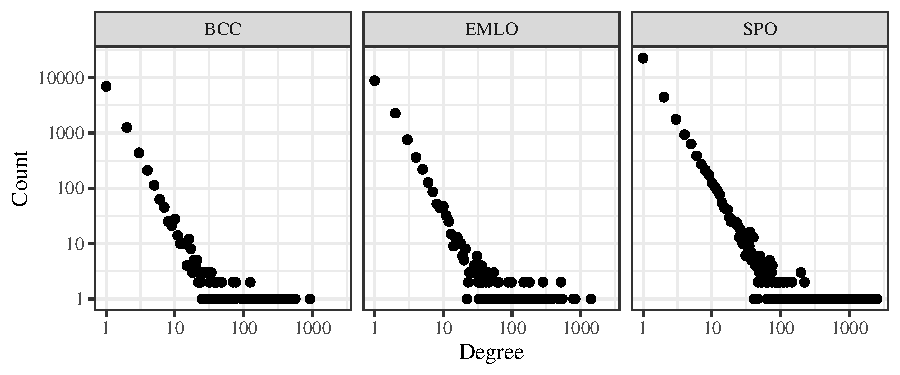
\includegraphics{network_robustness_article_anon_files/figure-latex/degreeDist-1.pdf}
\caption{\label{fig:degreeDist}Degree distribution plot for each of the networks. The downward-sloping diagonal line on a log-log axis plot is an indication that the networks are scale-free.}
\end{figure}

\hypertarget{sampling-techniques}{%
\subsection{Sampling techniques}\label{sampling-techniques}}

For each of the three networks, we created subsamples of the network by removing a) letters, b) nodes, c) years, d) folios, and e) entire correspondence catalogues, reflecting common forms of absences in the historical record, as discussed above. In all cases we removed a particular portion of the entity in question, e.g.~10\% of letters, or 30\% of catalogues, rounding up where necessary. As the volume of correspondence for individual years and in individual folios and catalogues varies considerably we expected larger fluctuations between samples in these cases than when removing a randomly selected set of individual letters.

Next, we compared the values of a set of standard metrics (total degree, betweenness centrality, eigenvector centrality, closeness centrality, and transitivity) in the full network to the equivalent values in the sampled networks for each node, disregarding any nodes that did not appear in the sample, similar to previous approaches in the literature.\footnote{Galaskiewicz, ``Estimating Point Centrality Using Different Network Sampling Techniques''; Costenbader and Valente, ``The Stability of Centrality Measures When Networks Are Sampled''; Stephen P. Borgatti, Kathleen M. Carley, and David Krackhardt, ``On the Robustness of Centrality Measures Under Conditions of Imperfect Data,'' \emph{Social Networks} 28, no. 2 (May 2006): 124--36, \url{https://doi.org/10.1016/j.socnet.2005.05.001}; Smith, Moody, and Morgan, ``Network Sampling Coverage II''; ``Network Science and Statistical Techniques for Dealing with Uncertainties in Archaeological Datasets.''} To compare the values we used Spearman's rank correlation (referred to \(\rho\) hereafter), because rankings are a more useful way for interpreting network metrics in many contexts, as absolute values may a) fluctuate due to larger historical developments and changes in archival practice, and b) are difficult to interpret in the case of betweenness centrality, closeness centrality, and eigenvector centrality, because the absolute values for the highest-ranking nodes can be orders of magnitude larger than the lowest-ranking for these measurements. We collected 100 independent samples at each 1\% interval, from 99\% to 1\% of the full network, for each category of removed entity (letter, folio, year, catalogue, and node). This process was repeated forty times to get a realistic average value and to measure variability. In other words, we simulated progressively increasing amounts of missing data, and measured how this affected quantitative results.

\begin{figure}
\centering
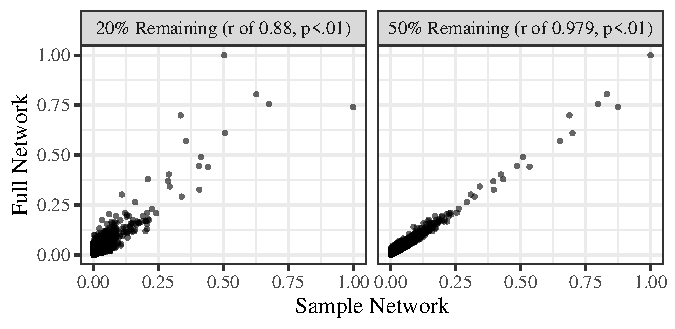
\includegraphics{network_robustness_article_anon_files/figure-latex/example-1.pdf}
\caption{\label{fig:example}Two example comparisons of eigenvector centrality scores, with 80\% and 50\% of letters removed at random.}
\end{figure}

\hypertarget{results}{%
\section{Results}\label{results}}

We find that the measures are remarkably robust to many types of data removal, across all of the networks. The figures 3 to 7 below display some of the key findings, and full results are available in the appendix, and in summarised form in table \ref{tab:summaryTable}. In each case we display the changes in correlation as larger parts of the network are removed as well as the variability of that change. The former is visualised in the charts below as a single blue line, representing the mean correlation for each sample (from 99\% to 1\%) and the latter is measured as the standard deviation of the forty observations for each sample, visualised as a gray shaded area. In general, most Spearman correlations remained high (many with a \(\rho\) above 0.7) until 50\% of the network was removed. Some metrics and sampling methods showed more variability than others, which is shown here through the standard deviation: for example, sampling catalogues resulted in high variance (a standard deviation of 0.328, where the possible values ranged from -1 to +1), and to a lesser extent, sampling years and nodes did too. Most network measures were robust to letter removal, and showed very little variability. This may be because of the particular structure of historical correspondence networks. In general, many connections between pairs of individuals will be marked by many letters, written over a number of years. This means that the most prominent connections in the network are also the most robust ones with regard to letter removal. Node removal produced similar results, though it resulted in more variation in measures that are calculated by using the entire network (closeness and eigenvector centralities). Surprisingly, even removing entire catalogues---essentially removing at random some of the top-scoring degree nodes---had little effect on the degree of the remaining nodes though it did have a more substantial impact on closeness and eigenvector centralities. We find that one metric, local clustering, is consistently sensitive to the removal of any type of data. This highlights that some research questions will be affected by incompleteness much more than others. It also underlines how remarkably robust most metrics actually are: the sensitivity of local clustering is the sensitivity that skeptics of quantitative analysis might expect to see across the board. We find that it is the exception that proves the rule, as local clustering demonstrates that some network metrics \emph{may} be very sensitive to data removal, but most are \emph{not}.

\begin{table}

\caption{\label{tab:summaryTable}Summary statistics for the removal correlations at twenty and fifty percent removed, showing the mean Spearman's rho ($\rho$) and standard deviation across forty iterations.}
\centering
\resizebox{\linewidth}{!}{
\begin{tabular}[t]{lrrrrrrrrr}
\toprule
\multicolumn{2}{c}{ } & \multicolumn{2}{c}{Catalogues} & \multicolumn{2}{c}{Letters} & \multicolumn{2}{c}{Nodes} & \multicolumn{2}{c}{Years} \\
\cmidrule(l{3pt}r{3pt}){3-4} \cmidrule(l{3pt}r{3pt}){5-6} \cmidrule(l{3pt}r{3pt}){7-8} \cmidrule(l{3pt}r{3pt}){9-10}
 & Portion removed & Mean $\rho$ & SD\textsuperscript{*} & Mean $\rho$ & SD & Mean $\rho$ & SD & Mean $\rho$ & SD\\
\midrule
\cellcolor{gray!6}{Betweenness Centrality\textsuperscript{\dag}} & \cellcolor{gray!6}{50} & \cellcolor{gray!6}{0.772} & \cellcolor{gray!6}{0.035} & \cellcolor{gray!6}{0.794} & \cellcolor{gray!6}{0.009} & \cellcolor{gray!6}{0.865} & \cellcolor{gray!6}{0.019} & \cellcolor{gray!6}{0.792} & \cellcolor{gray!6}{0.031}\\
Betweenness Centrality & 90 & 0.508 & 0.067 & 0.556 & 0.027 & 0.568 & 0.021 & 0.551 & 0.042\\
\cellcolor{gray!6}{Closeness Centrality} & \cellcolor{gray!6}{50} & \cellcolor{gray!6}{0.922} & \cellcolor{gray!6}{0.030} & \cellcolor{gray!6}{0.943} & \cellcolor{gray!6}{0.010} & \cellcolor{gray!6}{0.947} & \cellcolor{gray!6}{0.022} & \cellcolor{gray!6}{0.934} & \cellcolor{gray!6}{0.023}\\
Closeness Centrality & 90 & 0.669 & 0.175 & 0.789 & 0.038 & 0.717 & 0.091 & 0.716 & 0.095\\
\cellcolor{gray!6}{In-Degree} & \cellcolor{gray!6}{50} & \cellcolor{gray!6}{0.917} & \cellcolor{gray!6}{0.017} & \cellcolor{gray!6}{0.909} & \cellcolor{gray!6}{0.009} & \cellcolor{gray!6}{0.965} & \cellcolor{gray!6}{0.006} & \cellcolor{gray!6}{0.913} & \cellcolor{gray!6}{0.016}\\
\addlinespace
In-Degree & 90 & 0.751 & 0.059 & 0.724 & 0.012 & 0.845 & 0.034 & 0.744 & 0.032\\
\cellcolor{gray!6}{Out-Degree} & \cellcolor{gray!6}{50} & \cellcolor{gray!6}{0.878} & \cellcolor{gray!6}{0.028} & \cellcolor{gray!6}{0.881} & \cellcolor{gray!6}{0.016} & \cellcolor{gray!6}{0.933} & \cellcolor{gray!6}{0.011} & \cellcolor{gray!6}{0.883} & \cellcolor{gray!6}{0.023}\\
Out-Degree & 90 & 0.630 & 0.087 & 0.637 & 0.046 & 0.684 & 0.038 & 0.638 & 0.059\\
\cellcolor{gray!6}{Total Degree} & \cellcolor{gray!6}{50} & \cellcolor{gray!6}{0.843} & \cellcolor{gray!6}{0.030} & \cellcolor{gray!6}{0.832} & \cellcolor{gray!6}{0.010} & \cellcolor{gray!6}{0.903} & \cellcolor{gray!6}{0.011} & \cellcolor{gray!6}{0.839} & \cellcolor{gray!6}{0.023}\\
Total Degree & 90 & 0.636 & 0.064 & 0.650 & 0.022 & 0.663 & 0.033 & 0.646 & 0.030\\
\addlinespace
\cellcolor{gray!6}{Eigenvector Centrality} & \cellcolor{gray!6}{50} & \cellcolor{gray!6}{0.913} & \cellcolor{gray!6}{0.071} & \cellcolor{gray!6}{0.948} & \cellcolor{gray!6}{0.013} & \cellcolor{gray!6}{0.934} & \cellcolor{gray!6}{0.045} & \cellcolor{gray!6}{0.933} & \cellcolor{gray!6}{0.033}\\
Eigenvector Centrality & 90 & 0.639 & 0.224 & 0.810 & 0.054 & 0.643 & 0.183 & 0.706 & 0.147\\
\cellcolor{gray!6}{Local Clustering Coefficient} & \cellcolor{gray!6}{50} & \cellcolor{gray!6}{0.739} & \cellcolor{gray!6}{0.044} & \cellcolor{gray!6}{0.734} & \cellcolor{gray!6}{0.014} & \cellcolor{gray!6}{0.775} & \cellcolor{gray!6}{0.044} & \cellcolor{gray!6}{0.736} & \cellcolor{gray!6}{0.044}\\
Local Clustering Coefficient & 90 & 0.397 & 0.126 & 0.337 & 0.029 & 0.298 & 0.059 & 0.380 & 0.068\\
\bottomrule
\multicolumn{10}{l}{\rule{0pt}{1em}\textsuperscript{*} Standard deviation}\\
\multicolumn{10}{l}{\rule{0pt}{1em}\textsuperscript{\dag} Explanations of this and other standard network terms can be found in a glossary at the end of this article.}\\
\end{tabular}}
\end{table}

\hypertarget{letter-removal}{%
\subsection{Letter Removal}\label{letter-removal}}

Letter removal had surprisingly little effect on any of our three networks - the correlations stayed high (\(\rho\) above 0.6 in all three datasets) even when just 10\% of the total letters remained, and the variation between random samples was low (figure \ref{fig:lettersRemoval}). This is probably because of the aforementioned nature of correspondence data, in which many network edges are marked repeatedly, by many letters. Removing random letters when there are large numbers of them between two people makes it very unlikely the corresponding network edge disappears completely. There were some subtle differences between the metrics, in two broad patterns: some measurements, chiefly degree and betweenness centrality, became less correlated in an almost linear fashion as progressively larger parts of the network were removed, whereas eigenvector centrality showed very little difference until most of the network was removed, at which point it changed substantially. In all cases, the standard deviation was small: the values generated by each iteration stayed very close to the mean.

\begin{figure}

{\centering 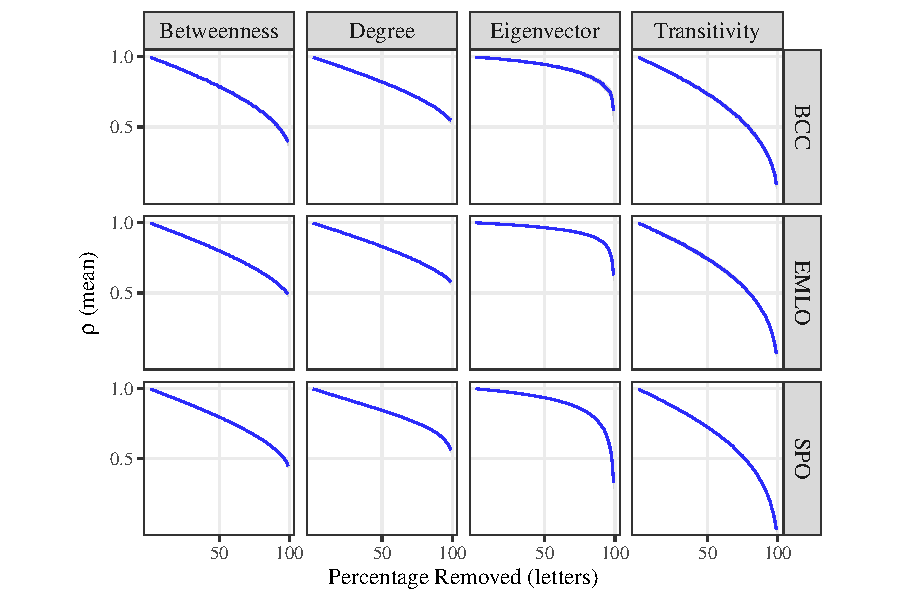
\includegraphics{network_robustness_article_anon_files/figure-latex/lettersRemoval-1} 

}

\caption{Robustness of Key Measures to Letter Removal. The blue line indicates the mean Spearman correlation ($\rho$) mean across all forty iterations. The standard deviation at each sample is represented as a shaded gray area, however it is usually not visible in this mode of removal because the variation between iterations was so small. Full results are in the appendix.}\label{fig:lettersRemoval}
\end{figure}

\hypertarget{node-removal}{%
\subsection{Node Removal}\label{node-removal}}

We assume that this method of data removal for historical networks is the least reflective of real-world missing historical data---most of the `important' actors within the networks are found across a number of archives, and it's unlikely (though not impossible, in some historical contexts) that an individual would be systematically erased across all archives, as both a sender and recipient of letters. There is existing literature which looks at the global tolerance of scale-free networks to both random error and coordinated attack, concluding that networks are robust to the former but vulnerable to the latter.\footnote{See Réka Albert, Hawoong Jeong, and Albert-László Barabási, ``Error and Attack Tolerance of Complex Networks,'' \emph{Nature} 406, no. 6794 (July 2000): 378--82, \url{https://doi.org/10.1038/35019019}; Petter Holme et al., ``Attack Vulnerability of Complex Networks,'' \emph{Phys. Rev. E} 65, no. 5 (May 2002): 056109, \url{https://doi.org/10.1103/PhysRevE.65.056109}; H. Jeong et al., ``Lethality and Centrality in Protein Networks,'' \emph{Nature} 411, no. 6833 (May 2001): 41--42, \url{https://doi.org/10.1038/35075138}.} This may partially explain why when random nodes are removed the individual network metrics are also resilient. Degree and betweenness sensitivity to node removal are very similar to the case of letter removal, with subtle differences. Node removal correlations are very high (\(\rho\) above 0.8) until 70\% of the network remains, and then decline more sharply than with letter removal (figure \ref{fig:nodesRemoval}). For closeness and eigenvector centrality, there is much more variation in the sensitivity across each iteration, as increasing portions of the network are removed. This may be because eigenvector and closeness centrality are more dependent on high-degree nodes, which are removed in larger numbers in these simulations than when letters are removed. The variation in eigenvector centrality scores is particularly striking for the BCC and EMLO networks, but less so for SPO.

\begin{figure}

{\centering 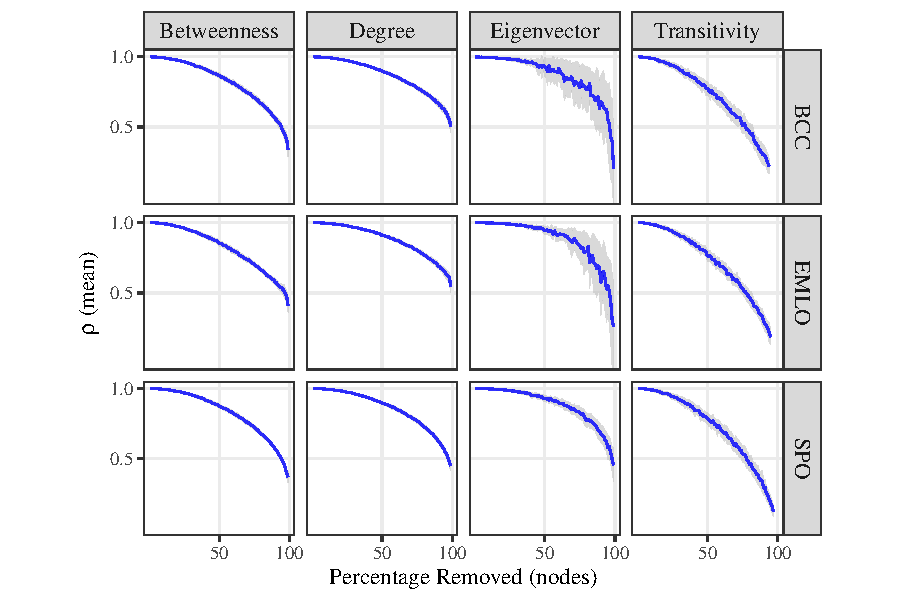
\includegraphics{network_robustness_article_anon_files/figure-latex/nodesRemoval-1} 

}

\caption{Robustness of Measures to Node Removal. The blue line indicates the mean Spearman correlation ($\rho$) across forty iterations. The standard deviation at each sample is represented as a shaded gray area. Generally, correlations remained high until 70\% of the network was removed and then declined sharply. Degree and betweeness sensitivity were similar to letter removal but closeness (not shown) and eigenvector centralities displayed more variation. Full results in the appendix.}\label{fig:nodesRemoval}
\end{figure}

\hypertarget{catalogue-removal}{%
\subsection{Catalogue removal}\label{catalogue-removal}}

One of the three archives studied here, EMLO, is divided into individual catalogues. Each of these catalogues is generally the correspondence of a single individual, often collected by an individual scholar. Because EMLO is organised, and new data is added to it, at a catalogue level, removing varying numbers of these catalogues may provide a realistic simulation of the impact of non-random missing (or added) data on historical scholarship. A common concern in historical network research is that a) any historical correspondence record is inevitably highly incomplete, and b) that many of the records that do survive have not yet been digitised, or even archived. In addition, the ongoing digitisation efforts mean that any analysed dataset will change over time as more correspondence is added to the digital archives. The question whether quantitative results obtained with current data will still hold after these future additions is therefore a further concern. The removal of catalogues can be used to examine the validity of the above concerns. While the results reveal larger variation between the independent simulations (due to the broad distribution of catalogue sizes), all network metrics are remarkably robust up to 50\% of removed catalogues (\(\rho\) above 0.8 in all cases except transivity and betweenness centrality) and on average not much less robust than for letter or node removal even for 90\% of removed catalogues (though in some simulations the correlation plummets for this percentage).

\begin{figure}

{\centering 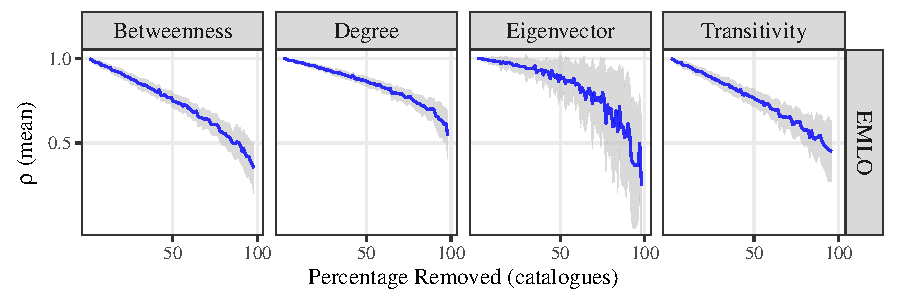
\includegraphics{network_robustness_article_anon_files/figure-latex/unnamed-chunk-13-1} 

}

\caption{Robustness of Measures to Catalogue Removal in EMLO dataset. Only EMLO has the catalogue as an organisational unit and so is displayed separately here. Removing full catalogues still did not have a large effect on correlations, though more variation between iterations was displayed - most likely because catalogue vary by size.  The blue line indicates the mean Spearman correlation ($\rho$) across all forty iterations. The standard deviation at each sample is represented as a shaded gray area. Full results in the appendix.}\label{fig:unnamed-chunk-13}
\end{figure}

\hypertarget{folio-removal}{%
\subsection{Folio Removal}\label{folio-removal}}

When we think of missing archival data, perhaps the first image that comes to mind is missing folios from shelves - these folios, as material objects, may go missing, be borrowed and not returned, be unavailable for digitisation because of conservation concerns, or destroyed, by accident or deliberately. Two of the archives here are organised by folio. The Bodleian card catalogue data comes from just over 500 individual manuscript folios - each containing anywhere from one to five hundred pieces of correspondence and the State Papers are organised similarly. Our algorithm simulates, essentially, walking the shelves of the archives at random and removing individual manuscript volumes, and calculates the effect on the resulting network measures.

When removing random samples of folios we find similar results to removing letters or nodes, with some results that highlights the organisation of the data. The eigenvector centrality measure of the BCC network shows high variability for random folio removal, which mirrors the pattern for node removal and may suggest that the way in which folios are organised affects the sensitivity of network measurements to random removal. For example, Bodleian card catalogue folios are more likely to contain the correspondence of a single individual, whereas in the State Papers, correspondence for important individuals is spread across a number of volumes. Historical network analysis, then, may be particularly sensitive to folio removal when an archive has been arranged by individual rather than, say, topic or date, though further investigation of this is needed.

\begin{figure}

{\centering 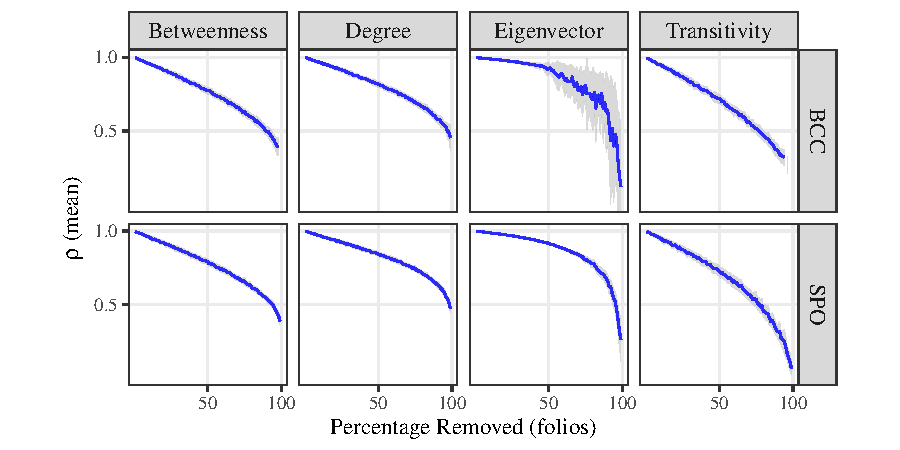
\includegraphics{network_robustness_article_anon_files/figure-latex/folio-1} 

}

\caption{Folio Removal results for BCC and SPO datasets. Blue line indicates the mean correlation score across all forty iterations. The standard deviation at each sample is represented as a shaded gray area. SPO and BCC include information on the source folio, and we used this as a unit to remove in sampling. Results differed as a result of the type of material collected in these folios: BCC folios are often person-based, and therefore show more variability, whereas SPO folios are often archived by subject or chronologically, and seem to display less variability}\label{fig:folio}
\end{figure}

\hypertarget{year-removal}{%
\subsection{Year removal}\label{year-removal}}

The three sample datasets, as seen in table \ref{tab:networkTable}, span large ranges of dates, sometimes three or four hundred years (though it should be noted that in all cases, the majority of records are found in a more limited timespan). Intuitively, it is entirely plausible that longitudinal historical datasets may be missing single or multiple years of data. EMLO, being a series of curated catalogues, is very much concentrated in a subset of the years it spans, but even a dataset like the State Papers has peaks and troughs across time. Diplomats often travelled for extensive periods of time, resulting in the dispersal of their correspondence. Joseph Williamson, the Under-secretary of State for the Southern Department of England between 1660 and 1674, travelled to Cologne to represent the State at a diplomatic conference for much of 1673 and 1674. Because of this, there is little correspondence involving Williamson for these years, and his dominance of the archive, due to his unprecendented personal effort in maintaining and archiving his working papers when in Whitehall, is such that this means there is a substantial dip in the volume of data during these years. In this case, the `missing' data is in fact dispersed elsewhere and therefore not a part of the State's archive, but one can imagine a similar scenario where the material could be simply lost. Data for particular years can be missing or relatively sparse for other more drastic reasons. During the English Civil War from 1642 to 1651, the complications arising from the split in the State's administration into a parliamentary and royalist dichotomy, compounded by the natural chaos of war meant that part of it moved its working papers elsewhere, and for these years again there is a substantial gap in the State Papers correspondence. A similar profile of variability in the volume of letters per year is also found in the EMLO dataset. Despite containing records spanning from approximately 1500 to 1800, the database coverage is uneven: two ten-year periods (1634-1644 and 1664-1673) contain 22.5\% of the total volume of letters. Because historical datasets are often longitudinal, ranging over a span of decades or centuries, substantial gaps in the temporal coverage become more likely and might be thought to have a great deal of effect on the resulting network. Results for this type of removed data largely mirror those for letter removal, with more variability for some metrics (as some years contain much more correspondence than others).

\begin{figure}

{\centering 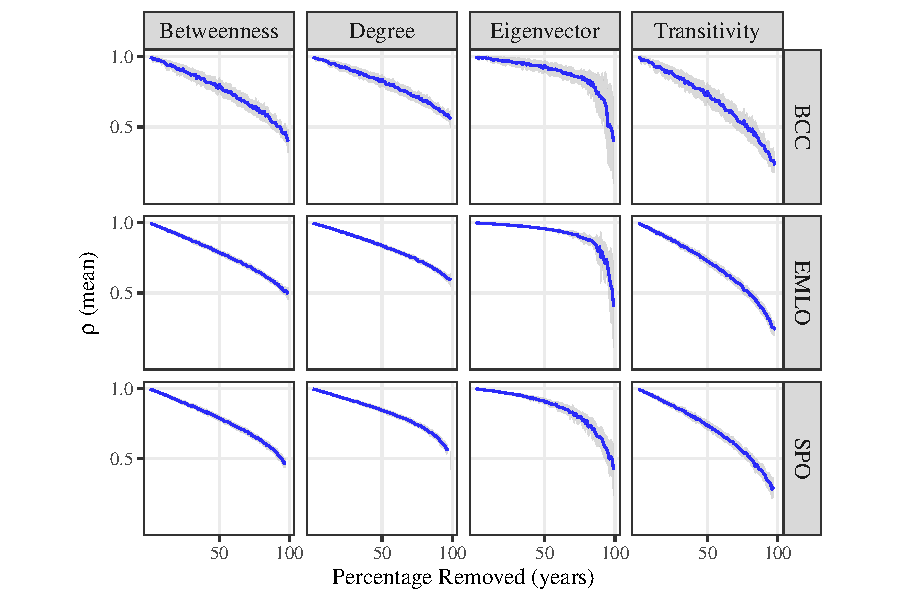
\includegraphics{network_robustness_article_anon_files/figure-latex/unnamed-chunk-14-1} 

}

\caption{Robustness of Measures to Year Removal. The blue line indicates the mean Spearman correlation score across all forty iterations. The standard deviation at each sample is represented as a shaded gray area. The results mirrored those of letter removal, with some more variability due to variations in the amount of material per year. Full results in the appendix)}\label{fig:unnamed-chunk-14}
\end{figure}

\hypertarget{conclusions}{%
\section{Conclusions}\label{conclusions}}

Historical network data (as indeed most network data - see Introduction) is always incomplete: this may be because of gaps in archives, the lack of digitisation, or simply because most communication is face-to-face and therefore leaves little record. There is a subset of more mundane `knowable' missing archival data, related in the first instance to its materiality as well as its editorial and digital afterlives: the missing data within it is from lost letters, burned books, uncalendared State papers, undigitised editions, uncrackable ciphers, and so forth which we can model and understand its impact on findings. Scholars working on correspondence have sometimes manually catalogued missing letters, and some of this data has been added to the EMLO database.\footnote{See \emph{The Correspondence of Henry Oldenburg}, ed. A. R. Hall and M. B. Hall, 13 vols (Madison, WI: University of Wisconsin Press; London: Mansel; London: Taylor \& Francis, 1965--86) and for a specific example from EMLO \url{https://tinyurl.com/y8lfdvha}} This reconstruction is valuable, which in itself brings more accuracy to quantitative historical network studies, but it is difficult. \emph{Modelling} the effect of missing letters, even if one cannot grasp their precise existence, is an enterprise which, as we have shown, is less time-consuming and can help to deal with the problem in the absence of reconstructed archives.

More specifically, modelling missing data and its effects on quantitative results can help to map and shape one's findings, tailored to the ways in which a particular dataset is sensitive to different results. Data curators might, for example, urge caution in the interpretation of eigenvector centrality or transitivity measures if it is thought that there are a large number of relevant catalogues which are yet to be digitised, and steer researchers towards another, more robust measurement instead. To this end, we have made available a user-friendly implementation of our code, which can be used to assess and compare the robustness of a set of network measures of any network. This application, developed using Shiny, allows a user to upload a simple network structure, an edge list, and run the same analyses as in this paper, specifying the type of missing data (currently nodes and letters are implemented), and the number of iterations to run (figure \ref{fig:screenshot}). If the edges have further attributes (folio or other source information) this can also be used as the basis for sampling, simply by selecting the attribute in a drop-down menu. It is hoped that this tool may also have applications outside of digital humanities. Furthermore, this technique could easily be adapted to allow for the removal of specific rather than random sections of the data, which could be used to assess the changes in a network's rankings were a particular individual, group, or time period to be removed.

\begin{figure}
\centering
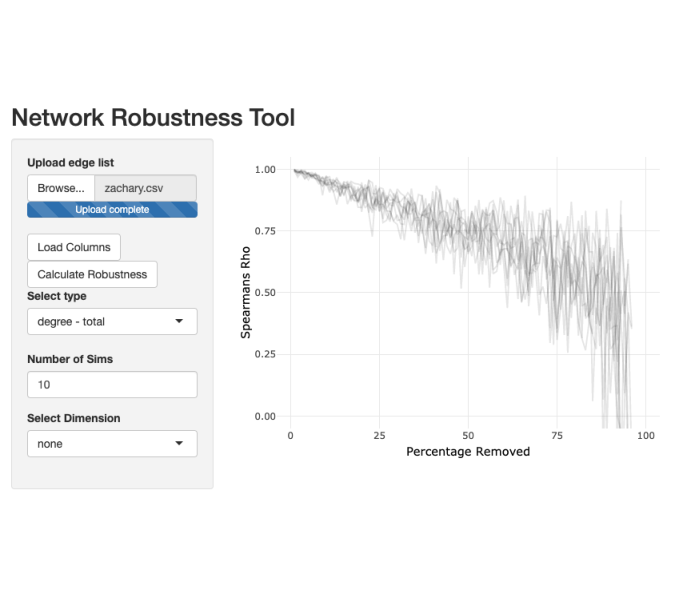
\includegraphics{network_robustness_article_anon_files/figure-latex/screenshot-1.pdf}
\caption{\label{fig:screenshot}Screenshot of Network Robustness Application, made with Shiny}
\end{figure}

The `archival turn' suggests that we should consider archives as multi-dimensional textual objects which need to be interpreted rather than neutral silos of documents to be mined for useful information. If this is the case, we should bring our quantitative toolsets and `read' them at scale much like the more traditional texts which are often the subject of digital humanities. This field has been much concerned with representativeness: Andrew Piper, arguing that because culture is `never finished', there should be a move away from thinking about `samples' and `bias' and towards what he terms representativeness: a mode which says that every part is a representation, and in which we focus on the curation of data rather than its quantity (or completeness). We suggest that an important facet of this data curation is to understand its missingness, and, moreover, where possible, the effect that this might have on resulting quantiative results, whether they be, as in this case, network metrics, but also more generally: the same technique might be applied to measures derived from work in Computational Literary Studies or Spatial Humanities.

Archival changes may be positive rather than negative. The acceleration of archival digitisation, projects to virtually reconstruct scattered archives, and the potential afforded by Handwritten Text Recognition mean that many of these unknown or uncertain links will increasingly come to light. The results in this paper suggest that quantitative analysis results of historical correspondence networks are largely robust to missing \emph{or added} data. Furthermore, the quantitative results discussed here typically operate at large scales and are most often a starting point for close reading and more detailed archival work. The robustness of the arguments that a scholar builds upon such results depends much more on the historical scholarship employed in their interpretation than on the incompleteness of the underlying data. It follows that historical argument must take archival absences into account, regardless of whether its foundations are quantitative or not.

\hypertarget{references}{%
\section*{References}\label{references}}
\addcontentsline{toc}{section}{References}

\hypertarget{refs}{}
\leavevmode\hypertarget{ref-ahnert_protestant_2015}{}%
Ahnert, Ruth, and Sebastian E. Ahnert. ``Protestant Letter Networks in the Reign of Mary I: A Quantitative Approach.'' \emph{ELH} 82, no. 1 (2015): 1--34. \url{https://doi.org/10.1353/elh.2015.0000}.

\leavevmode\hypertarget{ref-ahnert_metadata_2019}{}%
Ahnert, Ruth, and Sebastian E Ahnert. ``Metadata, Surveillance and the Tudor State.'' \emph{History Workshop Journal} 87 (April 2019): 27--51. \url{https://doi.org/10.1093/hwj/dby033}.

\leavevmode\hypertarget{ref-albert_error_2000}{}%
Albert, Réka, Hawoong Jeong, and Albert-László Barabási. ``Error and Attack Tolerance of Complex Networks.'' \emph{Nature} 406, no. 6794 (July 2000): 378--82. \url{https://doi.org/10.1038/35019019}.

\leavevmode\hypertarget{ref-barabasi_emergence_1999}{}%
Barabási, Albert-László, and Réka Albert. ``Emergence of Scaling in Random Networks.'' \emph{Science} 286, no. 5439 (n.d.): 509. \url{https://doi.org/10.1126/science.286.5439.509}.

\leavevmode\hypertarget{ref-bode_equivalence_2017}{}%
Bode, Katherine. ``The Equivalence of `Close' and `Distant' Reading; or, Toward a New Object for Data-Rich Literary History.'' \emph{Modern Language Quarterly} 78, no. 1 (March 2017): 77--106. \url{https://doi.org/10.1215/00267929-3699787}.

\leavevmode\hypertarget{ref-bonacich_factoring_1972}{}%
Bonacich, Phillip. ``Factoring and Weighting Approaches to Status Scores and Clique Identification.'' \emph{The Journal of Mathematical Sociology} 2, no. 1 (January 1972): 113--20. \url{https://doi.org/10.1080/0022250X.1972.9989806}.

\leavevmode\hypertarget{ref-bonacich_power_1987}{}%
---------. ``Power and Centrality: A Family of Measures.'' \emph{American Journal of Sociology} 92, no. 5 (March 1987): 1170--82. \url{https://doi.org/10.1086/228631}.

\leavevmode\hypertarget{ref-borgatti_robustness_2006}{}%
Borgatti, Stephen P., Kathleen M. Carley, and David Krackhardt. ``On the Robustness of Centrality Measures Under Conditions of Imperfect Data.'' \emph{Social Networks} 28, no. 2 (May 2006): 124--36. \url{https://doi.org/10.1016/j.socnet.2005.05.001}.

\leavevmode\hypertarget{ref-bourke_female_2017}{}%
Bourke, Evan. ``Female Involvement, Membership, and Centrality: A Social Network Analysis of the Hartlib Circle.'' \emph{Literature Compass} 14, no. 4 (April 2017). \url{https://doi.org/10.1111/lic3.12388}.

\leavevmode\hypertarget{ref-bozhilova_measuring_2019}{}%
Bozhilova, Lyuba V., Alan V. Whitmore, Jonny Wray, Gesine Reinert, and Charlotte M. Deane. ``Measuring Rank Robustness in Scored Protein Interaction Networks.'' \emph{BMC Bioinformatics} 20, no. 1 (December 2019): 446. \url{https://doi.org/10.1186/s12859-019-3036-6}.

\leavevmode\hypertarget{ref-costenbader_stability_2003}{}%
Costenbader, Elizabeth, and Thomas W Valente. ``The Stability of Centrality Measures When Networks Are Sampled.'' \emph{Social Networks} 25, no. 4 (October 2003): 283--307. \url{https://doi.org/10.1016/S0378-8733(03)00012-1}.

\leavevmode\hypertarget{ref-freeman_centrality_1979}{}%
Freeman, Linton C, Douglas Roeder, and Robert R Mulholland. ``Centrality in Social Networks: Ii. Experimental Results.'' \emph{Social Networks} 2, no. 2 (January 1979): 119--41. \url{https://doi.org/10.1016/0378-8733(79)90002-9}.

\leavevmode\hypertarget{ref-galaskiewicz_estimating_1991}{}%
Galaskiewicz, Joseph. ``Estimating Point Centrality Using Different Network Sampling Techniques.'' \emph{Social Networks} 13, no. 4 (December 1991): 347--86. \url{https://doi.org/10.1016/0378-8733(91)90002-B}.

\leavevmode\hypertarget{ref-holme_attack_2002}{}%
Holme, Petter, Beom Jun Kim, Chang No Yoon, and Seung Kee Han. ``Attack Vulnerability of Complex Networks.'' \emph{Phys. Rev. E} 65, no. 5 (May 2002): 056109. \url{https://doi.org/10.1103/PhysRevE.65.056109}.

\leavevmode\hypertarget{ref-jeong_lethality_2001}{}%
Jeong, H., S. P. Mason, A.-L. Barabási, and Z. N. Oltvai. ``Lethality and Centrality in Protein Networks.'' \emph{Nature} 411, no. 6833 (May 2001): 41--42. \url{https://doi.org/10.1038/35075138}.

\leavevmode\hypertarget{ref-leidwanger_manifesto_2014}{}%
Justin Leidwanger, Pascal Arnaud, Carl Knappett. ``A Manifesto for the Study of Ancient Mediterranean Maritime Networks.'' \emph{Antiquity} Project Gallery 88, no. 342 (October 2014). \url{http://journal.antiquity.ac.uk/projgall/leidwanger342}.

\leavevmode\hypertarget{ref-kossinets_effects_2006}{}%
Kossinets, Gueorgi. ``Effects of Missing Data in Social Networks.'' \emph{Social Networks} 28, no. 3 (July 2006): 247--68. \url{https://doi.org/10.1016/j.socnet.2005.07.002}.

\leavevmode\hypertarget{ref-laumann_boundary_1983}{}%
Laumann, Edward, Peter Marsden, and David Prensky. ``The Boundary Specification Problem in Network Analysis.'' \emph{Applied Network Analysis: A Methodological Introduction} 61 (January 1983).

\leavevmode\hypertarget{ref-lewis_ghosts_2013}{}%
Lewis, Miranda. ``Ghosts in the Machine: (Re)Constructing the Bodleian's Index of Literary Correspondence, 1927-1963.'' 2013. \url{http://www.culturesofknowledge.org/?p=295}.

\leavevmode\hypertarget{ref-lincoln_modeling_2020}{}%
Lincoln, Matthew, and Sandra Van Ginhoven. ``Modeling a Fragmented Archive: A Missing Data Case Study from Provenance Research,'' 2020, 25740302 Bytes. \url{https://doi.org/10.1184/R1/12363059.V1}.

\leavevmode\hypertarget{ref-malcolm_six_2001}{}%
Malcolm, Noel. ``Six Unknown Letters from Mersenne to Vegelin.'' \emph{The Seventeenth Century} 16, no. 1 (March 2001): 95--122. \url{https://doi.org/10.1080/0268117X.2001.10555485}.

\leavevmode\hypertarget{ref-noauthor_network_nodate}{}%
``Network Science and Statistical Techniques for Dealing with Uncertainties in Archaeological Datasets.'' Accessed September 16, 2020. \url{http://www.mattpeeples.net/netstats.html}.

\leavevmode\hypertarget{ref-penman_omnium_2016}{}%
Penman, Leigh T. I. ``Omnium Exposita Rapinæ: The Afterlives of the Papers of Samuel Hartlib.'' \emph{Book History} 19, no. 1 (2016): 1--65. \url{https://doi.org/10.1353/bh.2016.0000}.

\leavevmode\hypertarget{ref-scott_social_1988}{}%
Scott, John. ``Social Network Analysis.'' \emph{Sociology} 22, no. 1 (February 1988): 109--27. \url{https://doi.org/10.1177/0038038588022001007}.

\leavevmode\hypertarget{ref-smith_structural_2013}{}%
Smith, Jeffrey A., and James Moody. ``Structural Effects of Network Sampling Coverage I: Nodes Missing at Random.'' \emph{Social Networks} 35, no. 4 (October 2013): 652--68. \url{https://doi.org/10.1016/j.socnet.2013.09.003}.

\leavevmode\hypertarget{ref-smith_network_2017}{}%
Smith, Jeffrey A., James Moody, and Jonathan H. Morgan. ``Network Sampling Coverage II: The Effect of Non-Random Missing Data on Network Measurement.'' \emph{Social Networks} 48 (January 2017): 78--99. \url{https://doi.org/10.1016/j.socnet.2016.04.005}.

\leavevmode\hypertarget{ref-urbanek_comenius_2014}{}%
Urbánek, Vladimír. ``Comenius, the Unity of Brethren, and Correspondence Networks.'' \emph{Journal of Moravian History} 14, no. 1 (2014): 30--50. \url{http://www.jstor.org/stable/10.5325/jmorahist.14.1.0030}.

\leavevmode\hypertarget{ref-warren_six_2016}{}%
Warren, Christopher N., Daniel Shore, Jessica Otis, Lawrence Wang, Mike Finegold, and Cosma Shalizi. ``Six Degrees of Francis Bacon: A Statistical Method for Reconstructing Large Historical Social Networks.'' \emph{Digital Humanities Quarterly} 010, no. 3 (July 2016).

\leavevmode\hypertarget{ref-wasserman_social_1994}{}%
Wasserman, Stanley, and Katherine Faust. \emph{Social Network Analysis: Methods and Applications}. 1st ed. Cambridge University Press, 1994. \url{https://doi.org/10.1017/CBO9780511815478}.

\leavevmode\hypertarget{ref-strogatz_collective_1998}{}%
Watts, Duncan J., and Steven H. Strogatz. ``Collective Dynamics of `Small-World'networks.'' \emph{Nature} 393, no. 6684 (1998): 440--42. \url{https://doi.org/10.1038/30918}.

\newpage

\hypertarget{appendix}{%
\section*{Appendix}\label{appendix}}
\addcontentsline{toc}{section}{Appendix}

Additional results produced by the robustness analysis (including those used above), including in-degree, out-degree, and closeness centrality. As in the main plots, blue line indicates the mean and the limits of the gray area the standard deviation.

\hypertarget{full-results---early-modern-letters-online-emlo}{%
\subsection{Full Results - Early Modern Letters Online (EMLO)}\label{full-results---early-modern-letters-online-emlo}}

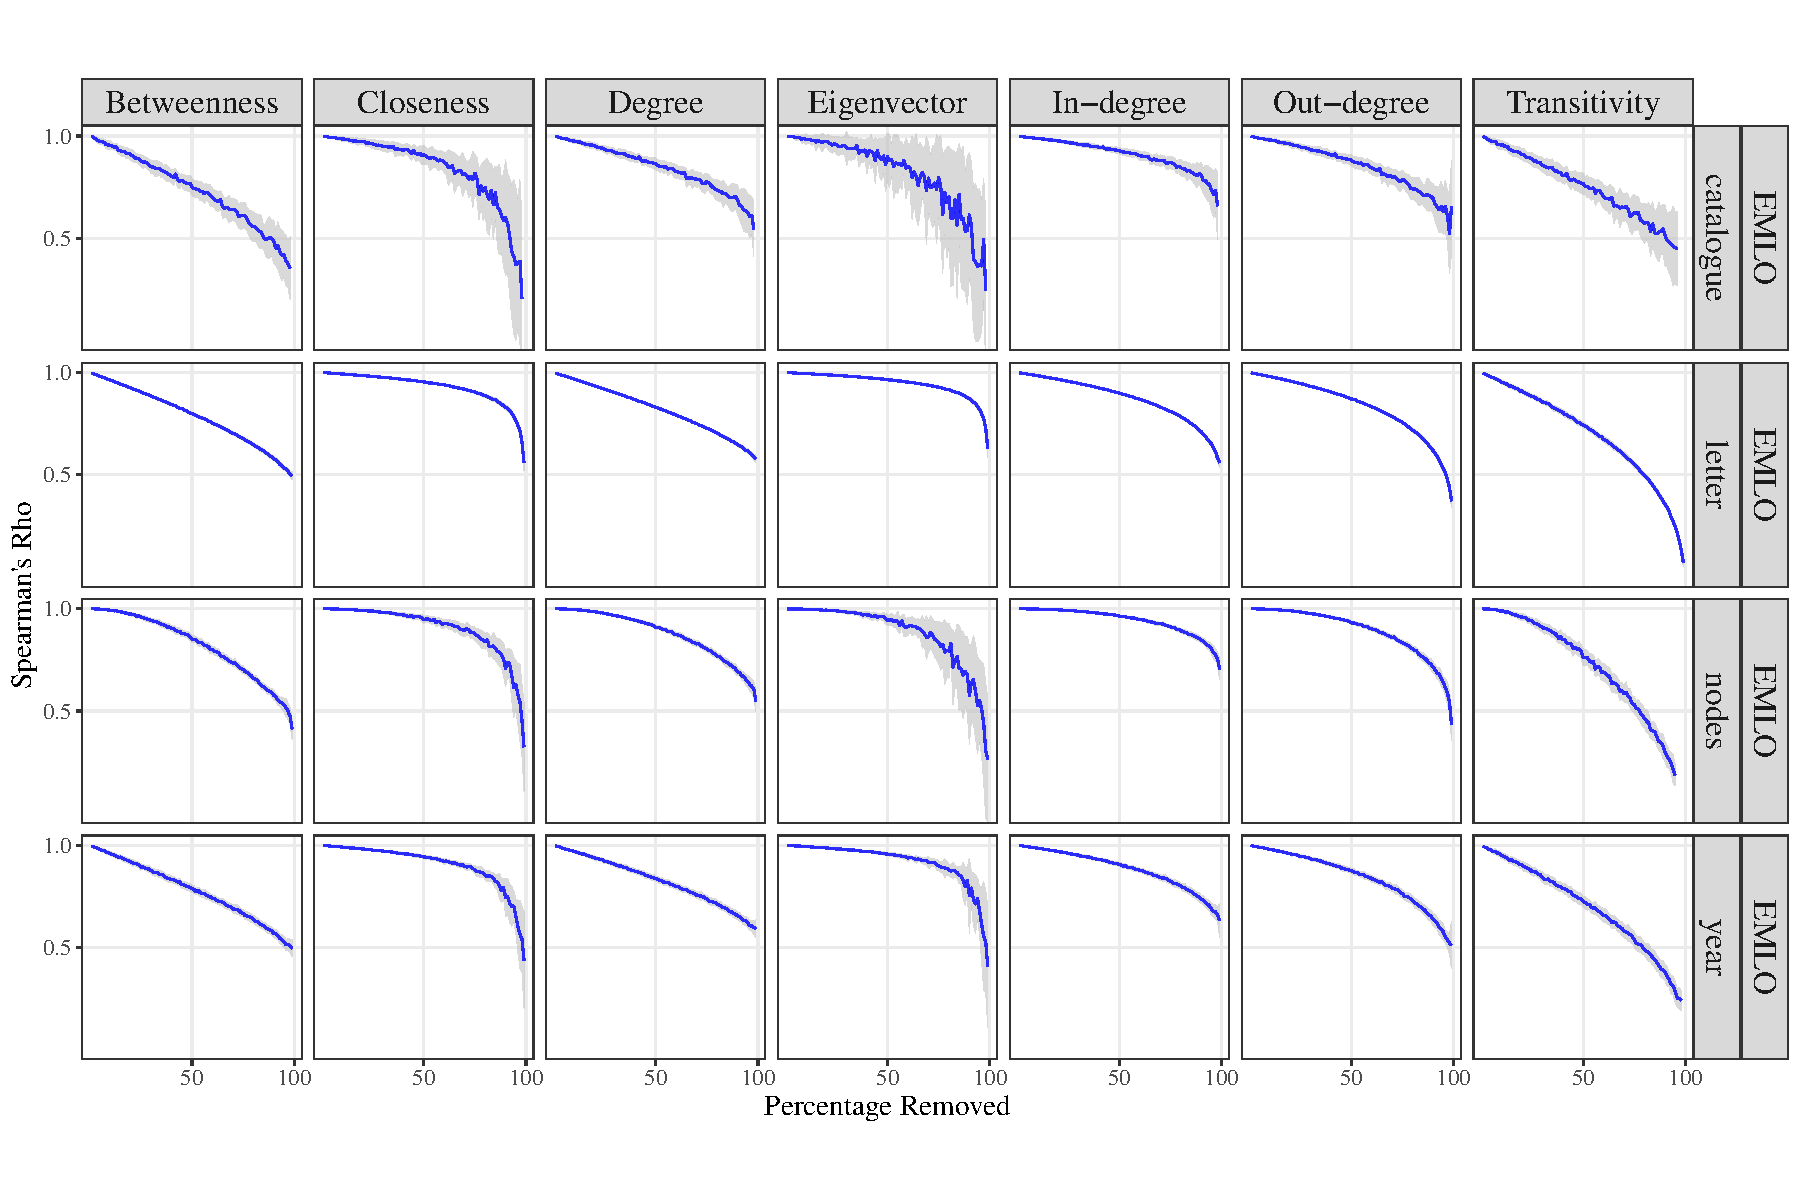
\includegraphics{network_robustness_article_anon_files/figure-latex/unnamed-chunk-15-1.pdf}
\newpage   

\hypertarget{full-results---state-papers-online-spo}{%
\subsection{Full Results - State Papers Online (SPO)}\label{full-results---state-papers-online-spo}}

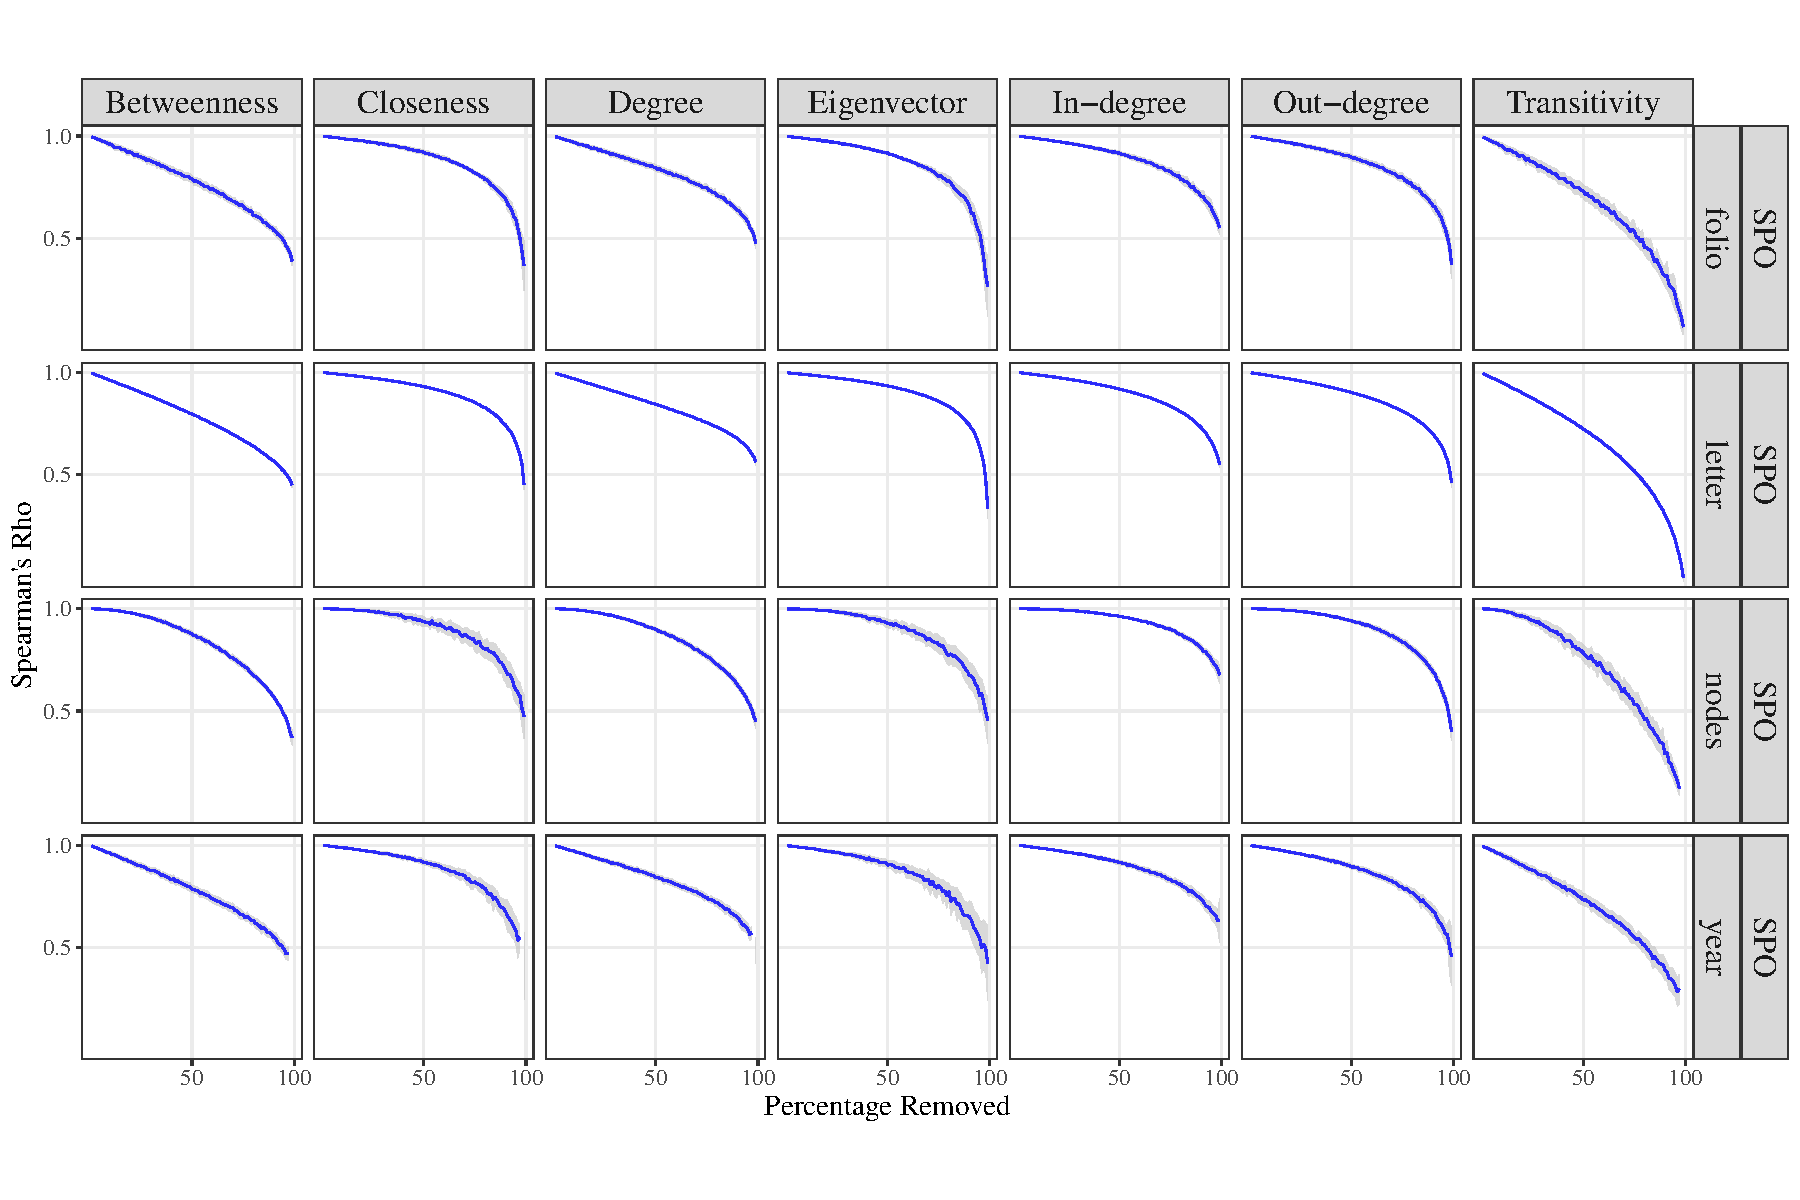
\includegraphics{network_robustness_article_anon_files/figure-latex/unnamed-chunk-16-1.pdf}

\newpage

\hypertarget{full-results---bodleian-card-catalogue-bcc}{%
\subsection{Full Results - Bodleian Card Catalogue (BCC)}\label{full-results---bodleian-card-catalogue-bcc}}

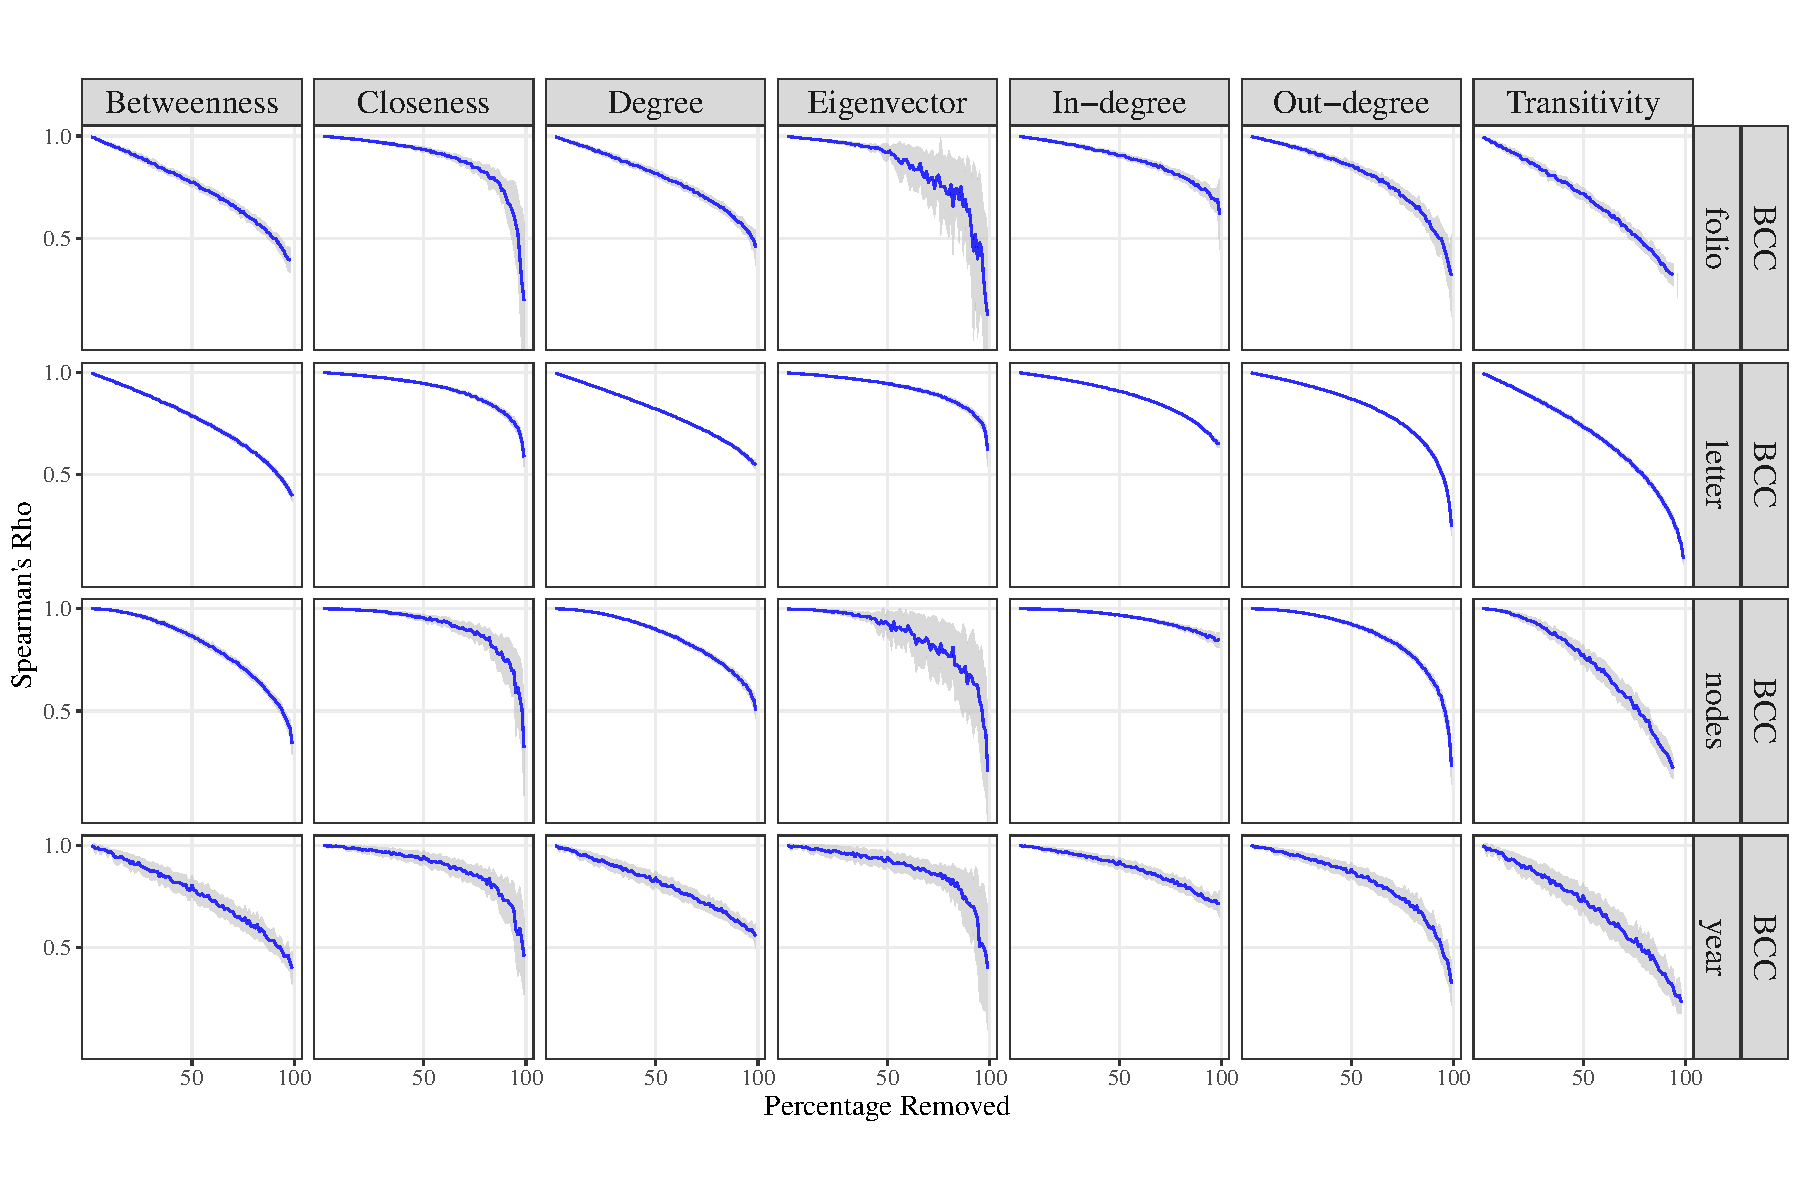
\includegraphics{network_robustness_article_anon_files/figure-latex/unnamed-chunk-17-1.pdf}

\end{document}
